
\documentclass{article}


\usepackage{lmodern}
\usepackage[german]{babel} 
\usepackage{csquotes}
\MakeOuterQuote{"} 

\usepackage{graphicx}
\usepackage{enumerate}

\usepackage{amssymb}
\usepackage{amsmath}
\usepackage{amsthm}
\usepackage{dsfont}
\usepackage{bm}

\usepackage{caption}
\usepackage{subcaption}
\usepackage{tikz}
\usetikzlibrary{cd}

\usepackage{hyperref}
\hypersetup{
	colorlinks  = true,
	urlcolor    = LMUpurple,
	linkcolor   = LMUgreen,
	citecolor   = LMUgreen
}
\usepackage[capitalize,nameinlink]{cleveref}
\Crefname{chapter}{Kapitel}{Kapitel}
\Crefname{section}{Abschnitt}{Abschnitte}
\Crefname{subsection}{Abschnitt}{Abschnitte}
\Crefname{figure}{Abbildung}{Abbildungen}
\Crefname{subfigure}{Abbildung}{Abbildungen}

\usepackage{bookmark}

\usepackage[landscape]{geometry}
\usepackage{url}
\usepackage{multicol}
\usepackage{esint}
\usetikzlibrary{decorations.pathmorphing}
\usepackage{colortbl}
\usepackage{xcolor}
\usepackage{mathtools}
\usepackage{listings}

\lstset{language=R,
    basicstyle=\small\ttfamily,
    stringstyle=\color{purple},
    otherkeywords={0,1,2,3,4,5,6,7,8,9},
    morekeywords={TRUE,FALSE},
    deletekeywords={data,frame,length,as,character},
    keywordstyle=\color{blue},
    commentstyle=\color{purple},
}


%\usepackage{blindtext}
\usepackage{subfiles}
\makeatletter


\usepackage{bm}
\usepackage{dsfont}

% blackboard bold 
\newcommand{\ind}{\mathds{1}}
\newcommand{\R}{\mathds{R}}
\newcommand{\N}{\mathds{N}}
\newcommand{\Q}{\mathds{Q}}
\providecommand{\C}{}
\renewcommand{\C}{\mathds{C}}
\providecommand{\P}{}
\renewcommand{\P}{\mathds{P}}
\newcommand{\Z}{\mathds{Z}}
\newcommand{\E}{\mathds{E}}
\newcommand{\K}{\mathds{K}}
\renewcommand{\L}{\mathds{L}}
\newcommand{\F}{\mathds{F}}
\providecommand{\G}{}
\newcommand{\D}{\mathds{D}}

% bold letters
\newcommand{\bnull}{\bm{0}}
\newcommand{\ba}{\bm{a}}
\newcommand{\bb}{\bm{b}}
\newcommand{\bc}{\bm{c}}
\newcommand{\bd}{\bm{d}}
\newcommand{\be}{\bm{e}}
% \newcommand{\bf}{\bm{f}}
\newcommand{\bg}{\bm{g}}
\newcommand{\bh}{\bm{h}}
\newcommand{\bi}{\bm{i}}
\newcommand{\bj}{\bm{j}}
\newcommand{\bk}{\bm{k}}
\newcommand{\bl}{\bm{l}}
% \newcommand{\bm}{\bm{m}}
\newcommand{\bn}{\bm{n}}
\newcommand{\bo}{\bm{o}}
\newcommand{\bp}{\bm{p}}
\newcommand{\bq}{\bm{q}}
\newcommand{\br}{\bm{r}}
\newcommand{\bs}{\bm{s}}
\newcommand{\bt}{\bm{t}}
\newcommand{\bu}{\bm{u}}
\newcommand{\bv}{\bm{v}}
\newcommand{\bw}{\bm{w}}
\newcommand{\bx}{\bm{x}}
\newcommand{\by}{\bm{y}}
\newcommand{\bz}{\bm{z}}

% bold letters
\newcommand{\bA}{\bm{A}}
\newcommand{\bB}{\bm{B}}
\newcommand{\bC}{\bm{C}}
\newcommand{\bD}{\bm{D}}
\newcommand{\bE}{\bm{E}}
% \newcommand{\bf}{\bm{f}}
\newcommand{\bG}{\bm{G}}
\newcommand{\bH}{\bm{H}}
\newcommand{\bI}{\bm{I}}
\newcommand{\bJ}{\bm{J}}
\newcommand{\bK}{\bm{K}}
\newcommand{\bL}{\bm{L}}
\newcommand{\bM}{\bm{M}}
\newcommand{\bN}{\bm{N}}
\newcommand{\bO}{\bm{O}}
\newcommand{\bP}{\bm{P}}
\newcommand{\bQ}{\bm{Q}}
\newcommand{\bR}{\bm{R}}
\newcommand{\bS}{\bm{S}}
\newcommand{\bT}{\bm{T}}
\newcommand{\bU}{\bm{U}}
\newcommand{\bV}{\bm{V}}
\newcommand{\bW}{\bm{W}}
\newcommand{\bX}{\bm{X}}
\newcommand{\bY}{\bm{Y}}
\newcommand{\bZ}{\bm{Z}}


% calligraphic letters
\newcommand{\Acal}{\mathcal{A}}
\newcommand{\Bcal}{\mathcal{B}}
\newcommand{\Ccal}{\mathcal{C}}
\newcommand{\Dcal}{\mathcal{D}}
\newcommand{\Ecal}{\mathcal{E}}
\newcommand{\Fcal}{\mathcal{F}}
\newcommand{\Gcal}{\mathcal{G}}
\newcommand{\Hcal}{\mathcal{H}}
\newcommand{\Ical}{\mathcal{I}}
\newcommand{\Jcal}{\mathcal{J}}
\newcommand{\Kcal}{\mathcal{K}}
\newcommand{\Lcal}{\mathcal{L}}
\newcommand{\Mcal}{\mathcal{M}}
\newcommand{\Ncal}{\mathcal{N}}
\newcommand{\Ocal}{\mathcal{O}}
\newcommand{\Pcal}{\mathcal{P}}
\newcommand{\Qcal}{\mathcal{Q}}
\newcommand{\Rcal}{\mathcal{R}}
\newcommand{\Scal}{\mathcal{S}}
\newcommand{\Tcal}{\mathcal{T}}
\newcommand{\Ucal}{\mathcal{U}}
\newcommand{\Vcal}{\mathcal{V}}
\newcommand{\Wcal}{\mathcal{W}}
\newcommand{\Xcal}{\mathcal{X}}
\newcommand{\Ycal}{\mathcal{Y}}
\newcommand{\Zcal}{\mathcal{Z}}

% greek letters
\newcommand{\eps}{\varepsilon}
\newcommand{\sd}{\sigma}
\newcommand{\ssd}{\sigma^2}
\newcommand{\hbe}{\hat{\beta}}
\newcommand{\beps}{\bm{\epsilon}}
\newcommand{\balpha}{\bm{\alpha}}
\newcommand{\bbeta}{\bm{\beta}}
\newcommand{\bchi}{\bm{\chi}}
\newcommand{\bdelta}{\bm{\delta}}
\newcommand{\bepsilon}{\bm{\epsilon}}
\newcommand{\bphi}{\bm{\phi}}
\newcommand{\bgamma}{\bm{\gamma}}
\newcommand{\betah}{\bm{\etah}}
\newcommand{\btheta}{\bm{\theta}}
\newcommand{\biota}{\bm{\iota}}
\newcommand{\bkappa}{\bm{\kappa}}
\newcommand{\blambda}{\bm{\lambda}}
\newcommand{\bmu}{\bm{\mu}}
\newcommand{\bnu}{\bm{\nu}}
\newcommand{\bomikron}{\bm{\omikron}}
\newcommand{\bpi}{\bm{\pi}}
\newcommand{\bxi}{\bm{\xi}}
\newcommand{\bzeta}{\bm{\zeta}}
\newcommand{\bomega}{\bm{\omega}}
% logic
\newcommand{\equivto}{\Leftrightarrow}
\newcommand{\quequiv}{\quad \equivto \quad}
\newcommand{\impl}{\Rightarrow}
\newcommand{\quimpl}{\quad \Rightarrow \quad}
\newcommand{\implby}{\Leftarrow}

% linear algebra
\newcommand{\tr}{\operatorname{tr}}
\newcommand{\spann}{\operatorname{span}}
\newcommand{\col}{\operatorname{col}}
\newcommand{\rang}{\operatorname{rang}}
\newcommand{\diag}{\operatorname{diag}}
\renewcommand{\vec}{\operatorname{vec}}
\newenvironment{roweqmat}[1]{\left(\array{@{}#1@{}}}{\endarray\right)}

\newcommand{\la}{\langle}
\newcommand{\ra}{\rangle}
\newcommand{\inner}[1]{\langle #1 \rangle}
\newcommand{\proj}{\operatorname{proj}}


\renewcommand{\bar}{\overline}

% statistics
\providecommand{\Pr}{}
\renewcommand{\Pr}{\mathbb{P}}
\newcommand{\var}{{\mathds{V}\mathrm{ar}}}
\newcommand{\bias}{{\operatorname{bias}}}
\newcommand{\abias}{{\mathrm{ABias}}}
\newcommand{\AMSE}{{\mathrm{AMSE}}}
\newcommand{\AMISE}{{\mathrm{AMISE}}}
\newcommand{\cov}{{\mathds{C}\mathrm{ov}}}
\newcommand{\corr}{{\mathrm{Corr}}}
\newcommand{\ov}{\overline}
\newcommand{\wh}[1]{\widehat{#1}}
\newcommand{\wt}[1]{\widetilde{#1}}
\newcommand{\tod}{\stackrel{d}{\to}}

\newcommand{\sumin}{\sum_{i = 1}^n}
\newcommand{\sumjn}{\sum_{j = 1}^n}


\newcommand{\KL}{\operatorname{KL}}
\DeclareMathOperator*{\argmin}{arg\,min}


\newcommand{\softmax}{\operatorname{SoftMax}}
\newcommand{\layernorm}{\operatorname{LayerNorm}}
\newcommand{\avg}{\operatorname{avg}}
\newcommand{\relu}{\operatorname{ReLu}}

% figure environment with scaling in multiples of \textwidth
\newcommand{\fig}[1][1]{
  \includegraphics[width = #1\textwidth]
}

% footnote without mark
\makeatletter
\def\blfootnote{\gdef\@thefnmark{}\@footnotetext}
\makeatother

\newcommand{\envbreak}{ \, \\[-12pt]}
\newcommand{\tw}{\textwidth}


% Sonstiges
%\newcommand*\bigcdot{\mathpalette\bigcdot@{.5}}
%\newcommand*\bigcdot@[2]{\mathbin{\vcenter{\hbox{\scalebox{#2}{$\m@th#1\bullet$}}}}}
\newcommand{\hr}{\centerline{\rule{3.5in}{1pt}}}

\definecolor{mycolor}{HTML}{3C8031}
\newcommand{\tc}[1]{\textcolor{red}{#1}}


\makeatother

\title{Lineare Algebra für Statistiker Cheat Sheet}


\advance\topmargin-.8in
\advance\textheight3in
\advance\textwidth3in
\advance\oddsidemargin-1.5in
\advance\evensidemargin-1.5in
\parindent0pt
\parskip2pt

\begin{document}

% Dokumente einfügen


\section*{Kapitel 1 - Das einfache lineare Regressionsmodell}

\begin{multicols*}{3}

\tikzstyle{mybox} = [draw=black, fill=white, very thick,
    rectangle, rounded corners, inner sep=10pt, inner ysep=10pt]
\tikzstyle{fancytitle} =[fill=black, text=white, font=\bfseries]



%------------ Einfaches lineares Regressionsmodell ---------------
\begin{tikzpicture}
\node [mybox] (box){%
    \begin{minipage}{0.3\textwidth}
    Das \tc{einfache lineare Regressionsmodell} hat die Form 
    $$Y_i = \beta_0 + \beta_1 x_i + \eps_i,\quad i = 1, \dots, n$$
    für ein festes numerisches $x_i$ und $\eps_i \sim \Ncal(0,\ssd)$.
    Beachte, dass per Definition gilt $Y_i| x_i \sim \Ncal(\beta_0 + \beta_1 x_i, \ssd)$
    \end{minipage}
};
%------------ Einfaches lineares Regressionsmodell Header ---------------------
\node[fill = black, text=white, font=\bfseries, right=10pt] at (box.north west) 
{Einfaches lineares Regressionsmodell};
\end{tikzpicture}

%------------ KQ Schätzer ---------------
\begin{tikzpicture}
\node [mybox] (box){%
    \begin{minipage}{0.3\textwidth}
    Wir schätzen die Parameter $(\beta_0, \beta_1)$ durch 
    \begin{align}
        (\hbe0, \hbe1) = \argmin_{(\beta_0, \beta_1)} \sum_{i = 1}^n(Y_i - (\beta_0 + \beta_1 x_i))^2
    \end{align}
    und nennen $(\hbe0, \hbe1)$ den \tc{KQ-Schätzer von $(\beta_0, \beta_1)$} und 
    $\hat{\eps}_i := Y_i - (\hbe0 + \hbe1 x_i)$ die \tc{Residuen}.
    \end{minipage}
};
%------------ KQ Schätzer Header ---------------------
\node[fill = black, text=white, font=\bfseries, right=10pt] at (box.north west) 
{Kleinste Quadrate (KQ) Schätzer};
\end{tikzpicture}

%------------ Existenz und Berechnung vom KQ Schätzer ---------------
\begin{tikzpicture}
\node [mybox] (box){%
    \begin{minipage}{0.3\textwidth}
    Der KQ-Schätzer existiert und ist eindeutig, falls $\sum_{i = 1}^n (x_i - \bar{x})^2 \neq 0$. 
    Dieser lässt sich berechnen als 
    \begin{align*}
        \hbe1 = & \quad \frac{S_{xY}}{S_x^2} = 
        \frac{\frac1n\sum_{i = 1}^n (x_i - \bar{x})(Y_i - \bar{Y})}{\frac1n\sum_{i = 1}^n (x_i - \bar{x})^2}\\
        \hbe0 = & \quad \bar{Y} - \hbe1 \bar{x}.
    \end{align*}
    Durch differenzieren von der Gleichung (1) erhält man $(\hbe0, \hbe1)$ als Lösung der 
    \tc{Normalengleichungen}
    \begin{align*}
        \sumin \hat{\eps}_i = 0\\
        \sumin \hat{\eps}_i x_i = 0
    \end{align*}
    \end{minipage}
};
%------------ Existenz und Berechnung vom KQ Schätzer Header --------
\node[fill = purple, text=white, font=\bfseries, right=10pt] at (box.north west) 
{Existenz und Berechnung vom KQ Schätzer};
\end{tikzpicture}


%------------ Interpretation der Modellparameter ---------------
\begin{tikzpicture}
    \node [mybox] (box){%
        \begin{minipage}{0.3\textwidth}
        Für $Y_i = \gb0 + \gb1 x_i + \eps_i \quad ,i = 1,\dots,n$
        mit \\$\E(Y_i|x_i) = \gb0 + \gb1x_i$ gilt,
        \begin{itemize}
            \item wenn $x$ um eine \textbf{Einheit} steigt, 
            dann steigt $Y$ \textbf{im Erwartungswert} um $\beta_1$ Einheiten.
            \item Es gilt $\beta_0 = \E(Y|X = 0)$.
            \item Der Parameter $\sd$ die erwartete Abweichung der $Y_i$-Werte von der Regressionsgerade an.
        \end{itemize}
        \end{minipage}
    };
%------------ Interpretation der Modellparameter Header ---------------------
\node[fill = blue, text=white, font=\bfseries, right=10pt] at (box.north west) {Interpretation der Modellparameter};
\end{tikzpicture}
    

%------------ Eigenschaften des KQ-Schätzers ---------------
\begin{tikzpicture}
    \node [mybox] (box){%
        \begin{minipage}{0.3\textwidth}
        Gegeben dem einfachen linearen Modell, gilt für den KQ-Schätzer $(\hbe0,\hbe1)$
        \begin{itemize}
            \item Erwartungstreue: $\E(\hbe0,\hbe1) = (\gb0,\gb1)$.
            \item $\V(\hbe1) = \frac{\ssd}{nS_x^2}$ und $\V(\hbe0) = \ssd (\frac 1n + \frac{\bar{x}^2}{nS_x^2})$.
            \item $(\hbe0,\hbe1)$ ist der maximum-likelihood Schätzer.
        \end{itemize}
        \end{minipage}
    };
%------------ Eigenschaften des KQ-Schätzers Header ---------------------
\node[fill = purple, text=white, font=\bfseries, right=10pt] at (box.north west) {Eigenschaften des KQ-Schätzers};
\end{tikzpicture}


%------------ Schätzer für $\ssd$ ---------------
\begin{tikzpicture}
    \node [mybox] (box){%
        \begin{minipage}{0.3\textwidth}
        Gegeben dem einfachen linearen Modell mit\\$\eps_i \sim \Ncal(0,\ssd)$, gilt
        $$\hat{\sd}^2 := \frac{1}{n-2}\sumin \hat{\eps}_i^2$$ 
        ist ein erwartungstreuer Schätzer von $\ssd$ und 
        $$\frac{n-2}{\ssd}\hat{\sd}^2 \sim \chi_{n-2}^2.$$
        Der KQ-Schätzer $(\hbe0,\hbe1)$ und der Schätzer $\hat{\sd}^2$ sind stoch.unabhängig.
        \end{minipage}
    };
    %------------ Schätzer für $\ssd$ Header ---------------------
    \node[fill = purple, text=white, font=\bfseries, right=10pt] at (box.north west) {Schätzer für $\ssd$};
    \end{tikzpicture}
    


%------------ Konfidenzintervalle für $\gb0$ und $\gb1$ ---------------
\begin{tikzpicture}
    \node [mybox] (box){%
        \begin{minipage}{0.3\textwidth}
        Gegeben dem einfachen linearen Modell mit\\$\eps_i \sim \Ncal(0,\ssd)$, gilt für $\hbe1$ und $\hbe0$
        $$\frac{\hbe1 - \gb1}{\hat{\sd}_{\hbe1}} \sim t_{n-2} \text{ mit } \hat{\sd}_{\hbe1} 
        := \sqrt{\frac{\hat{\sd}^2}{\sumin (x_i - \bar{x})^2}}$$
        $$\frac{\hbe0 - \gb0}{\hat{\sd}_{\hbe0}} \sim t_{n-2} \text{ mit } \hat{\sd}_{\hbe0} 
        := \sqrt{\hat{\sd}^2 \frac{\sumin x_i^2}{n\sumin (x_i - \bar{x})^2}}$$
        Damit können wir Konfidenzintervalle zum Niveau $1 - \alpha$ für $\gb1$ und $\gb0$ erzeugen:
        $$[\ \hbe1 - \hat{\sd}_{\hbe1}t_{1 - \alpha/2}(n-2); \hbe1 + \hat{\sd}_{\hbe1}t_{1 - \alpha/2}(n-2) ]\ $$
        $$ [\ \hbe0 - \hat{\sd}_{\hbe0}t_{1 - \alpha/2}(n-2); \hbe0 + \hat{\sd}_{\hbe0}t_{1 - \alpha/2}(n-2) ]\ $$
        \end{minipage}
    };
    %------------  Konfidenzintervalle für $\gb0$ und $\gb1$ Header ---------------------
    \node[fill = purple, text=white, font=\bfseries, right=10pt] at (box.north west) 
    {Konfidenzintervalle für $\gb0$ und $\gb1$};
    \end{tikzpicture}

%------------ Quadratsummenzerlegung ---------------
\begin{tikzpicture}
    \node [mybox] (box){%
        \begin{minipage}{0.3\textwidth}
        Gegeben sei ein einfaches linearen Modell mit\\$\eps_i \sim \Ncal(0,\ssd)$ und 
        $\hat{Y}_i := \hbe0 + \hbe1x_i$. Dann gilt
        $$ \underbrace{\sumin (Y_i - \bar{Y})^2}_{\text{SST}} = \underbrace{\sumin (Y_i - \hat{Y}_i)^2}_{\text{SSE}} 
        - \underbrace{\sumin(\hat{Y}_i - \bar{Y})^2}_{\text{SSM}} .$$
        \begin{align*}
            & \text{SST(otal):} & \text{Gesamtstreuung von Y}\\
            & \text{SSE(rror):} & \text{Streuung der Residuen}\\
            & \text{SSM(odel):} & \text{Streuung, die das Modell erklärt}\\
        \end{align*}
        \end{minipage}
    };
%------------ Quadratsummenzerlegung Header ---------------------
\node[fill = purple, text=white, font=\bfseries, right=10pt] at (box.north west) {Quadratsummenzerlegung};
\end{tikzpicture}
    
%------------ Bestimmtheitsmaß ---------------
\begin{tikzpicture}
    \node [mybox] (box){%
        \begin{minipage}{0.3\textwidth}
        Unter Verwendung der obigen Notation definieren wir das \tc{Bestimmtheitsmaß} als
        $$R^2 = \frac{\text{SSM}}{\text{SST}} = 1 - \frac{\text{SSE}}{\text{SST}}.$$
        Es gilt $$R^2 = r_{xY}^2 = \frac{S_{xY}}{S_xS_Y},$$
        wobei $r_{xY}$ der Bravais-Pearson Korrel.koeffizient ist.
        \end{minipage}
    };
    %------------ Bestimmtheitsmaß Header ---------------------
    \node[fill = black, text=white, font=\bfseries, right=10pt] at (box.north west) {Bestimmtheitsmaß};
    \end{tikzpicture}

%------------ Interpretation von R^2 ---------------
\begin{tikzpicture}
    \node [mybox] (box){%
        \begin{minipage}{0.3\textwidth}
        \begin{itemize}
            \item $R^2$ beschreibt den Anteil der Varianz von $Y$, die durch $x$ erklärt wird.
            \item $R$ ist invariant gegenüber linearen linearen Transformationen von $x$ und $Y$.
            \item $R$ ist symmetrisch bzgl. $x$ und $Y$.
            \item \tc{!} $R^2$ hängt auch von der Streuung von $x$ in der Stichprobe ab.
        \end{itemize}
        \end{minipage}
    };
%------------ Interpretation von R^2 Header ---------------------
\node[fill = blue, text=white, font=\bfseries, right=10pt] at (box.north west) {Interpretation von $R^2$};
\end{tikzpicture}



%------------ Prognosewert ---------------
\begin{tikzpicture}
    \node [mybox] (box){%
        \begin{minipage}{0.3\textwidth}
        Gegeben sei ein einfaches linearen Modell mit\\$\eps_i \sim \Ncal(0,\ssd)$ und 
        $\hat{Y}_i := \hbe0 + \hbe1x_i, \quad i = 1,\dots,n$. 
        Sei nun eine weitere Beobachtung $x_{n+1}$ mit zugehörigem 
        $Y_{n + 1} = \gb0 + \gb1 x_{n + 1} + \eps_{n + 1}$ gegeben. Der \tc{Prognosewert von $Y_{n+1}$} 
        ist definiert als $\hat{Y}_{n + 1} = \hbe0 + \hbe1 x_{n + 1}$
        \end{minipage}
    };
    %------------ Prognosewert Header ---------------------
    \node[fill = black, text=white, font=\bfseries, right=10pt] at (box.north west) 
    {Prognosewert};
    \end{tikzpicture}
    

%------------ Prognosefehler ---------------
\begin{tikzpicture}
    \node [mybox] (box){%
        \begin{minipage}{0.3\textwidth}
        Gegeben sei ein einfaches linearen Modell, sowie eine weitere Beobachtung $x_{n+1}$ mit zugehörigem 
        $Y_{n + 1}$ sowie der Prognosewert $\hat{Y}_{n + 1}$. Dann gilt
        \begin{align*}
            \E(\hat{Y}_{n + 1} - Y_{n + 1}) = {} & 0 \\
            \V(\hat{Y}_{n + 1} - Y_{n + 1}) = {} & 
            \ssd \Bigr[ 1 + \frac 1n + \frac{(x_{n + 1} - \bar{x})^2}{\sumin (x_i - \bar{x})^2} \Bigr]
        \end{align*}
        \end{minipage}
    };
    %------------ Prognosefehler Header ---------------------
\node[fill = purple, text=white, font=\bfseries, right=10pt] at (box.north west) 
{Prognosefehler};
\end{tikzpicture}


%------------ Prognoseintervall ---------------
\begin{tikzpicture}
\node [mybox] (box){%
    \begin{minipage}{0.3\textwidth}
    Gegeben sei ein einfaches linearen Modell, sowie eine weitere Beobachtung $x_{n+1}$ mit zugehörigem 
    $Y_{n + 1}$ sowie der Prognosewert $\hat{Y}_{n + 1}$. Dann können wir für $Y_{n + 1}$ ein 
    Konfidenzintervall zum Niveau $1 - \alpha$ konstruieren:
    $$[\ \hat{Y}_{n+1} - \hat{\sd}_{\hat{Y}_{n+1}}t_{1 - \alpha/2}(n-2); 
    \hat{Y}_{n+1} + \hat{\sd}_{\hat{Y}_{n+1}}t_{1 - \alpha/2}(n-2) ]\ $$
    mit $$\hat{\sd}_{\hat{Y}_{n+1}} = \hat{\sd}^2 \Bigr[ 1 + \frac 1n + \frac{(x_{n + 1} - 
    \bar{x})^2}{\sumin (x_i - \bar{x})^2} \Bigr].$$
    \end{minipage}
};
%------------ Prognoseintervall Header ---------------------
\node[fill = purple, text=white, font=\bfseries, right=10pt] at (box.north west) {Prognoseintervall};
\end{tikzpicture}


%------------ R-Code ---------------
\begin{tikzpicture}
\node [mybox] (box){%
    \begin{minipage}{0.3\textwidth}
    \begin{lstlisting}
# simuliere aus einfachem lin. Modell
beta0 <- 3
beta1 <- 1
sigma <- 2
x <- seq(from = 0, to = 10, by = 0.5)
e <- rnorm(length(x), sd = sigma)
y <- beta0 + beta1 * x + e
dat <- data.frame(x, y)

# Lineares Modell erzeugen
reg = lm(y ~ x, data = dat)
summary(reg)

# Konfidenzintervalle
confint(reg, level = 0.95)

    \end{lstlisting}
    \end{minipage}
};
%------------ R-Code Header ---------------------
\node[fill = olive, text=white, font=\bfseries, right=10pt] at (box.north west) {R-Code};
\end{tikzpicture}

%------------ Interpretation von transformierten Modellen ---------------
\begin{tikzpicture}
    \node [mybox] (box){%
        \begin{minipage}{0.3\textwidth}
        \begin{itemize}
            \item Log-Log-Modell: $$\log(Y_i) = \gb0 + \gb1 \log(x_i) + \eps_i$$
            Wenn $x_i$ um den Faktor $a$ steigt, dann steigt $Y_i$ im Erwartungswert um
            den Faktor $a^{\gb1} = e^{\gb1 log(a)}$.\\
            Alternativ: Wenn $x_i$ um 1\% steigt, dann steigt $Y_i$ im Erwartungswert um $(e^{\gb1 log(1.01)} - 1)$\%.
            \item Linear-Log-Modell:  $$Y_i = \gb0 + \gb1 \log(x_i) + \eps_i$$
            Wenn $x_i$ um $p$\% steigt, dann steigt $Y_i$ im Erwartungswert um $\gb1 \cdot \log(1 + p)\%$.\\
            Alternativ: Wenn $x_i$ um 1\% steigt, dann steigt $Y_i$ im Erwartungswert um approximativ $\gb1$ Einheiten.
            \item Log-Linear-Modell: $$\log(Y_i) = \gb0 + \gb1 x_i + \eps_i$$
            Wenn $x_i$ um eine Einheit steigt, dann steigt $Y_i$ im Erwartungswert um den Faktor $e^{\gb1}$.
        \end{itemize}
        
        
        \end{minipage}
    };
    %------------  Interpretation von transformierten Modellen Header ---------------------
    \node[fill = blue, text=white, font=\bfseries, right=10pt] at (box.north west) {Interpretation von transformierten Modellen};
    \end{tikzpicture}


%------------ Vorlesung ---------------
\begin{tikzpicture}
\node [mybox] (box){%
    \begin{minipage}{0.3\textwidth}
    $R^2$ ist abhängig von $X$. Das heißt über mehrere Studien hinweg, die das gleiche messen, ist
    $R^2$ nur vergleichbar, wenn auch $X$ vergleichbar ist. Je sichererer wir mit unserem Schätzer sein
    wollen, desto höher sollten wir die Varianz von $X$ einstellen. Gegeben, dass der Zusammenhang tatsächlich linear
    ist, würde eine höhere Varianz von $X$ zu einer geringeren Varianz von $\hbe1$ führen.\\

    Im multiplen Reg.modell ist es KEINE Annahme, dass $x_i, x_j$ unabhängig voneinander sind.
    Es wäre nur praktisch für die Interpretation der Effekte. Das "magische" am multiplen Reg.modell
    ist, dass ich für verschiedene Größen kontrollieren/korrigieren kann.\\

    Erwartungstreue gilt auch bei abhängigkeit und normalverteilt ist nicht nötig.
    Varianzformel benötigt unabhängigkeit.
    \end{minipage}
};
%------------ Überschrift Header ---------------------
\node[fill = black, text=white, font=\bfseries, right=10pt] at (box.north west) {Vorlesung};
\end{tikzpicture}






% %------------ Überschrift ---------------
% \begin{tikzpicture}
% \node [mybox] (box){%
%     \begin{minipage}{0.3\textwidth}
    
%     \end{minipage}
% };
% %------------ Überschrift Header ---------------------
% \node[fill = black, text=white, font=\bfseries, right=10pt] at (box.north west) {Überschrift};
% \end{tikzpicture}







\end{multicols*}
\section*{Kapitel 2 - Das multiple lineare Regressionsmodell}

\begin{multicols*}{3}

\tikzstyle{mybox} = [draw=black, fill=white, very thick, rectangle, rounded
    corners, inner sep=10pt, inner ysep=10pt] \tikzstyle{fancytitle}
    =[fill=black, text=white, font=\bfseries]




%------------ multiple lineare Regressionsmodell ---------------
\begin{tikzpicture}
    \node [mybox] (box){%
        \begin{minipage}{0.3\textwidth}
        Das \tc{multiple lineare Regressionsmodell} hat die Form
        $$Y_i = \underbrace{\gb0 + \gb1 x_{i1} + \dots + \gb{p}
        x_{ip}}_{\bx_i^\top = (1, x_{i1}, \dots, x_{ip})} + \eps_i; i =
        1,\dots,n$$ oder in Matrix-Vektor Notation: $\bY = \bX \bbeta + \beps$
        mit \\
        $ \bY = \begin{pmatrix} Y_1 \\ \vdots \\ Y_n \end{pmatrix} , \bX =
            \begin{pmatrix} 1 & x_{11} & \dots & x_{1p} \\
            \vdots & \vdots & \ddots & \vdots \\
            1 & x_{n1} & \dots & x_{np} \end{pmatrix} ,\\
        \bbeta = \begin{pmatrix} \gb0 \\ \vdots \\ \gb{p} \end{pmatrix} , \beps
            = \begin{pmatrix} \eps_1\\ \vdots \\ \eps_n \end{pmatrix}$.\\
        Wir nehmen dabei an, dass $\bX \in \R^{n \times (p+1)}$ eine feste
        Design-Matrix mit vollem Rang ist und dass\\$\beps \sim \Ncal(\bm0, \ssd
        \bI)$. Wir definieren \tc{$p' := p+1$}.
        \end{minipage}
    };
%------------ multiple lineare Regressionsmodell Header ---------------------
\node[fill = black, text=white, font=\bfseries, right=10pt] at (box.north west)
{Multiples lineares Regressionsmodell};
\end{tikzpicture}
    
%------------ KQ Schätzer ---------------
\begin{tikzpicture}
\node [mybox] (box){%
    \begin{minipage}{0.3\textwidth}
    Wir schätzen den Parameter(vektor) $\bbeta$ durch 
    \begin{align}
        \hbbeta = \argmin_{\bbeta \in \mathds{R}^{p'}} (\bY - \bX \bbeta)^\top (\bY - \bX \bbeta)
    \end{align}
    und nennen $\hbbeta$ den \tc{KQ-Schätzer von $\bbeta$} und \\
    $\hat{\eps}_i := Y_i - \bx_i^\top \hbbeta$ die \tc{Residuen}.
    \end{minipage}
};
%------------ KQ Schätzer Header ---------------------
\node[fill = black, text=white, font=\bfseries, right=10pt] at (box.north west)
{Kleinste Quadrate (KQ) Schätzer};
\end{tikzpicture}
    
    
%------------ Existenz und Berechnung vom KQ Schätzer ---------------
\begin{tikzpicture}
\node [mybox] (box){%
    \begin{minipage}{0.3\textwidth}
    Der KQ-Schätzer existiert und ist eindeutig, falls $\bX^\top\bX$
    invertierbar ist. Dieser lässt sich berechnen als 
    \begin{align*}
        \hbbeta = (\bX^\top\bX)^{-1} \bX^\top \bY
    \end{align*}
    Durch differenzieren von der Gleichung (2) erhält man $\hbbeta$ als Lösung
    der 
    \tc{Normalengleichung}
    \begin{align*}
        \bX^\top \hbeps = 0
    \end{align*}
    \end{minipage}
};
%------------ Existenz und Berechnung vom KQ Schätzer Header --------
\node[fill = purple, text=white, font=\bfseries, right=10pt] at (box.north west)
{Existenz und Berechnung vom KQ Schätzer};
\end{tikzpicture}

%------------ Gauss-Markov-Theorem ---------------
\begin{tikzpicture}
    \node [mybox] (box){%
        \begin{minipage}{0.3\textwidth}
        Sei das Modell $\bY = \bX \bbeta + \beps$ gegeben mit $\E(\beps) = \bm0$
        und $\Cov(\beps) = \ssd \bI$. Dann ist der KQ-Schätzer $\hbbeta$ der
        beste lineare erwartungstreue Schätzer (best linear unbiased estimator,
        BLUE) von $\bbeta$.
        
        Das heißt, dass für jeden anderen linearen erwartungstreuen Schätzer
        $\tilde{\bbeta}$ von $\bbeta$ gilt $\V(\hbbeta) \leq
        \V(\tilde{\bbeta})$.
        \end{minipage}
    };
    %------------ Gauss-Markov-Theorem Header --------
    \node[fill = purple, text=white, font=\bfseries, right=10pt] at (box.north
    west) {Gauss-Markov-Theorem};
    \end{tikzpicture}

%------------ Interpretation der Modellparameter ---------------
\begin{tikzpicture}
    \node [mybox] (box){%
        \begin{minipage}{0.3\textwidth}
        \begin{itemize}
            \item \tc{ceteris paribus}: alle anderen x-Variablen bleiben
            konstant.
            \item (Theoretische) Interpretation: Steigt $x_k$ um eine Einheit,
            so steigt $Y$ (ceteris paribus) im Erwartungswert um $\beta_k$
            Einheiten.
            \item (Empirische) Interpretation: Steigt $x_k$ um eine Einheit, so
            steigt $Y$ (ceteris paribus) im Durchschnitt um $\hbe{k}$ Einheiten.
            \item \tc{!} $\gb{k}$ charakterisiert den Einfluss von $x_k$ unter
            Berücksichtigung der übrigen Variablen (Confounder-Korrektur). Das
            heißt, dass in einem einfachen linearen Regressionsmodell mit $Y_i =
            \gb0 + \gb{k}' x_{ik} + \eps_i$ wäre im Allgemeinen $\gb{k}' \neq
            \gb{k}$.
        \end{itemize}
        \end{minipage}
    };
%------------ Interpretation der Modellparameter Header ---------------------
\node[fill = blue, text=white, font=\bfseries, right=10pt] at (box.north west)
{Interpretation der Modellparameter};
\end{tikzpicture}

%------------ Eigenschaften des KQ-Schätzers ---------------
\begin{tikzpicture}
    \node [mybox] (box){%
        \begin{minipage}{0.3\textwidth}
        Gegeben dem multiplen linearen Modell, gilt für den KQ-Schätzer
        $\hbbeta$
        \begin{itemize}
            \item Erwartungstreue: $\E(\hbbeta) = \bbeta$. \\
            \tc{!} Gilt auch ohne die Annahme $\beps \sim \Ncal(\bm0, \ssd
            \bI)$, solange $\E(\beps) = \bm0$
            \item $\V(\hbbeta) = \ssd (\bX^\top\bX)^{-1}$.\\
            \tc{!} Gilt auch ohne die Annahme $\beps \sim \Ncal(\bm0, \ssd
            \bI)$, solange $\Cov(\beps) = \ssd \bI$
            \item $\hbbeta \sim \Ncal(\bbeta,\ssd (\bX^\top\bX)^{-1})$
        \end{itemize}
        \end{minipage}
    };
%------------ Eigenschaften des KQ-Schätzers Header ---------------------
\node[fill = purple, text=white, font=\bfseries, right=10pt] at (box.north west)
{Eigenschaften des KQ-Schätzers};
\end{tikzpicture}

%------------ Hat-Matrix und Residualmatrix ---------------
\begin{tikzpicture}
    \node [mybox] (box){%
        \begin{minipage}{0.3\textwidth}
        Gegeben dem multiplen linearen Modell mit\\$\rang(\bX) = p'$ gilt
        \begin{align*}
        \hbY := & \bX\underbrace{(\bX^\top\bX)^{-1} \bX^\top \bY}_{\hbbeta} \\
        \bP :=  & \underbrace{\bX(\bX^\top\bX)^{-1} \bX^\top}_{n \times n} \\
        \hbeps = & \bY - \hbY = (\bI - \bP)\bY\\
        \bQ := & \bI - \bP
        \end{align*}
        $\bP$ heißt \tc{Hat-Matrix} und $\bQ$ heißt \tc{Residualmatrix}.
        \end{minipage}
    };
%------------ Hat-Matrix und Residualmatrix Header ---------------------
\node[fill = black, text=white, font=\bfseries, right=10pt] at (box.north west)
{Hat-Matrix und Residualmatrix};
\end{tikzpicture}

%------------ Geometrische Interpretation Hat-Matrix und Residualmatrix
%---------------
\begin{tikzpicture}
    \node [mybox] (box){%
        \begin{minipage}{0.3\textwidth}
        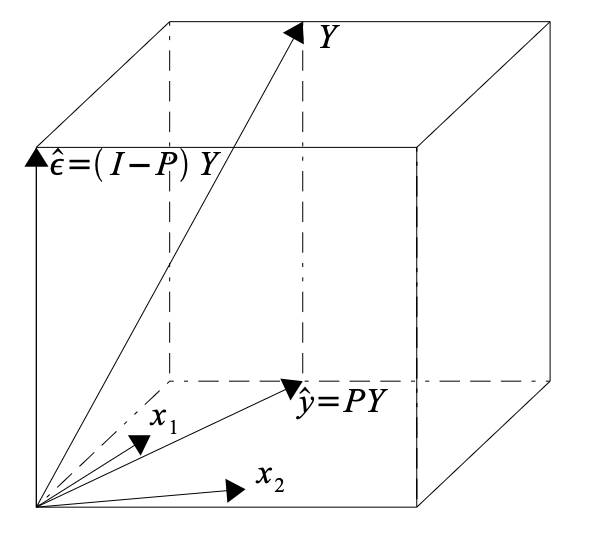
\includegraphics[scale=0.7]{fig/Projektion.png}\\
        Die KQ-Schätzung ist eine orthogonale Projektion von $\bY$ auf den von
        den $\bx$-Vektoren aufgespannten Unterraum.
        \end{minipage}
    };
%------------ Geometrische Interpretation Hat-Matrix und Residualmatrix Header
%---------------------
\node[fill = blue, text=white, font=\bfseries, right=10pt] at (box.north west)
{Geometrische Interpretation};
\end{tikzpicture}


%------------ Eigenschaften der Hat-Matrix und Residualmatrix ---------------
\begin{tikzpicture}
    \node [mybox] (box){%
        \begin{minipage}{0.3\textwidth}
        Die Hat-Matrix $\bP$ und die Residualmatrix $\bQ$ sind
        Projektionsmatrizen und zueinander orthogonal:
        \begin{align*}
        &\bP^\top = \bP \text{ und } \bP^2 = \bP \\
        &\bQ^\top = \bQ \text{ und }  \bQ^2 = \bQ \\
        &\bP\bQ = \bQ\bP = \bm0.
        \end{align*}
        Daraus folgt
        \begin{align*}
        &\V(\hbY) = \ssd \bP \\
        &\V(\hbeps) = \ssd \bQ, \text{ da } \hbeps = \bQ\beps
        \end{align*}
        \end{minipage}
    };
%------------ Eigenschaften der Hat-Matrix und Residualmatrix Header
%---------------------
\node[fill = purple, text=white, font=\bfseries, right=10pt] at (box.north west)
{Eigenschaften von $\bP$ und $\bQ$};
\end{tikzpicture}


%------------ Schätzer für $\ssd$ ---------------
\begin{tikzpicture}
    \node [mybox] (box){%
        \begin{minipage}{0.3\textwidth}
        Gegeben dem multiplen linearen Modell, gilt
        $$\hat{\sd}^2 := \frac{\hbeps^\top\hbeps}{n-p'} = \frac{1}{n-p'}
        \sumin \hat{\eps}_i^2$$ ist ein erwartungstreuer Schätzer von $\ssd$.\\
        \tc{!} Gilt auch ohne die Annahme $\beps \sim \Ncal(\bm0, \ssd \bI)$,
        solange $\E(\beps) = \bm0$ und $\Cov(\beps) = \ssd \bI$
        \end{minipage}
    };
%------------ Schätzer für $\ssd$ Header ---------------------
\node[fill = purple, text=white, font=\bfseries, right=10pt] at (box.north west)
{Schätzer für $\ssd$};
\end{tikzpicture}
    


% %------------ Überschrift ---------------
% \begin{tikzpicture}
%     \node [mybox] (box){%
%         \begin{minipage}{0.3\textwidth}
        
%         \end{minipage}
%     };
% %------------ Überschrifts Header ---------------------
% \node[fill = black, text=white, font=\bfseries, right=10pt] at (box.north west) {Überschrift};
% \end{tikzpicture}
    
\end{multicols*}
\section*{Kapitel 3 - Quadratsummenzerlegung und statistische Inferenz im multiplen linearen Regressionsmodell}

\begin{multicols*}{3}

\tikzstyle{mybox} = [draw=black, fill=white, very thick,
    rectangle, rounded corners, inner sep=10pt, inner ysep=10pt]
\tikzstyle{fancytitle} =[fill=black, text=white, font=\bfseries]



%------------ Quadratsummenzerlegung ---------------
\begin{tikzpicture}
    \node [mybox] (box){%
        \begin{minipage}{0.3\textwidth}
        Gegeben sei das multiple lineare Regressionsmodell mit
        $\rang(\bX) = p'$. Dann gilt
        \footnotesize{
        $$
        \underbrace{(\bY - \bar\bY)^\top (\bY - \bar\bY)}_{SST} =
        \underbrace{(\bY - \hbY)^\top (\bY - \hbY)}_{SSE} + 
        \underbrace{(\hbY - \bar\bY)^\top (\hbY - \bar\bY)}_{SSM}.
        $$}

        \begin{align*}
        & \text{SST(otal):} & & \text{Gesamt-Quadratsumme (korrigiert)}\\
        & \text{SSE(rror):} & &\text{Fehler-Quadratsumme}\\
        & \text{SSM(odel):} & &\text{Modell-Quadratsumme}\\
        \end{align*}
        \end{minipage}
    };
%------------ Quadratsummenzerlegung Header ---------------------
\node[fill = purple, text=white, font=\bfseries, right=10pt] at (box.north west) {Quadratsummenzerlegung};
\end{tikzpicture}
    
\end{multicols*}
\section*{Kapitel 4 - Diskrete Einflußgrößen}

\begin{multicols*}{3}

\tikzstyle{mybox} = [draw=black, fill=white, very thick,
    rectangle, rounded corners, inner sep=10pt, inner ysep=10pt]
\tikzstyle{fancytitle} =[fill=black, text=white, font=\bfseries]



%------------ Kodierung ---------------
\begin{tikzpicture}
    \node [mybox] (box){%
        \begin{minipage}{0.3\textwidth}
        Sei $C$ eine nominale Variable mit $K$ Ausprägungen.
        \vspace{0.5cm}

        \tc{\textbf{Dummy-Kodierung:}}\\
         Wir definieren $K$ neue Variablen $Z_1, \dots, Z_K$ als
         $$Z_k(C) = \begin{cases} 1, & \text{falls } C = k \\ 0, & \text{sonst} \end{cases}$$
         $Z_1, \dots, Z_K$ sind abhängig, da $Z_K = 1 - \sum_{k=1}^{K-1} Z_k$
        \vspace{0.5cm}

        \tc{\textbf{Effekt-Kodierung:}}
        Wir definieren $K-1$ neue Variablen $Z_1^e, \dots, Z_{K-1}^e$ als
        $$Z_k^e(C) = \begin{cases} 1, & \text{falls } C = k \\ -1, & \text{falls } C = K \\ 0, & \text{sonst} \end{cases}$$
        Note: $Z_k(\bC) = \begin{pmatrix}
            Z_k(C_1) \\ \vdots \\ Z_k(C_n) \end{pmatrix}$ und $Z_k^e(\bC) = \begin{pmatrix}
                Z_k^e(C_1) \\ \vdots \\ Z_k^e(C_n) \end{pmatrix}$
    \end{minipage}
    };
%------------ Kodierung Header ---------------------
\node[fill = black, text=white, font=\bfseries, right=10pt] at (box.north west) 
{Kodierung};
\end{tikzpicture}

%------------ Setup einfache Varianzanalyse ---------------
\begin{tikzpicture}
    \node [mybox] (box){%
        \begin{minipage}{0.3\textwidth}
        Im folgenden betrachten wir die einfache Varianzanalyse mit nur einer diskreten Einflußgröße 
        $\bC = \begin{pmatrix} C_1 \\ \vdots \\ C_n \end{pmatrix}$ mit $K$ Ausprägungen.
        Sei $n_k$ dabei die Anzahl der Beobachtungen mit $C_i = k$.
        \end{minipage}
    };
%------------ Setup einfache Varianzanalyse Header ---------------------
\node[fill = black, text=white, font=\bfseries, right=10pt] at (box.north west) 
{Setup einfache Varianzanalyse};
\end{tikzpicture}


%------------ Mittelwertsmodell ---------------
\begin{tikzpicture}
    \node [mybox] (box){%
        \begin{minipage}{0.3\textwidth}
        Das \tc{Mittelwertsmodell} ist gegeben durch
        $$Y_{k_l} = \mu_k + \epsilon_{k_l} \quad l = 1,\dots, n_k \quad k = 1,\dots,K$$
        oder in Matrix-Vektor Notation: 
        $$\bY = (Z_1(\bC) \dotsm Z_K(\bC)) \begin{pmatrix}
            \mu_1 \\ \vdots \\ \mu_K
        \end{pmatrix} + \bepsilon$$
        Bei dem Mittelwertsmodell gibt es keinen Intercept und die $\mu_k$ sind die Mittelwerte der $k$-ten Gruppe.
        Der Effekt der $k$-ten Gruppe ist also $\mu_k$.
        \end{minipage}
    };
%------------ Mittelwertsmodell Header ---------------------
\node[fill = black, text=white, font=\bfseries, right=10pt] at (box.north west) 
{Mittelwertsmodell};
\end{tikzpicture}

%------------ Mittelwertsmodell Beispiel ---------------
\begin{tikzpicture}
    \node [mybox] (box){%
        \begin{minipage}{0.3\textwidth}
        Für $K = 3$ Ausprägungen und $n_k = 2$ für alle $k=1,2,3$ erhalten wir als Mittelwertsmodell:
        $$\bY = \begin{pmatrix} Y_{1_1} \\ Y_{1_2} \\ Y_{2_1} \\ Y_{2_2} \\ Y_{3_1} \\ Y_{3_2}
         \end{pmatrix} = \begin{pmatrix}
            1 & 0 & 0 \\ 1 & 0 & 0 \\ 0 & 1 & 0 \\ 0 & 1 & 0 \\ 0 & 0 & 1 \\ 0 & 0 & 1 \end{pmatrix} \begin{pmatrix}
                \mu_1 \\ \mu_2 \\ \mu_3 \end{pmatrix} + \begin{pmatrix}
                    \eps_{1_1} \\ \eps_{1_2} \\ \eps_{2_1} \\ \eps_{2_2} \\ \eps_{3_1} \\ \eps_{3_2}
        \end{pmatrix}$$
        \end{minipage}
    };
%------------ Mittelwertsmodell Beispiel Header ---------------------
\node[fill = blue, text=white, font=\bfseries, right=10pt] at (box.north west) 
{Mittelwertsmodell Beispiel};
\end{tikzpicture}


%------------ Modell mit Effekt-Kodierung ---------------
\begin{tikzpicture}
    \node [mybox] (box){%
        \begin{minipage}{0.3\textwidth}
        Das \tc{Modell mit Effekt-Kodierung} ist gegeben durch
        $$Y_{k_l} = \mu + \tau_k + \epsilon_{k_l}; \quad \tau_K = -\sum_{k = 1}^{K-1} \tau_k$$ 
        für $\quad l = 1,\dots, n_k \quad k = 1,\dots,K$
        oder in Matrix-Vektor Notation: 
        $$\bY = (\be \hspace{2mm} Z_1^e(\bC) \dotsm Z_{K-1}^e(\bC)) \begin{pmatrix}
            \mu \\ \tau_1 \\ \vdots \\ \tau_{K-1}
        \end{pmatrix} + \bepsilon$$
        Bei dem Modell mit Effekt-Kodierung gibt es einen Intercept $\mu$ und die $\tau_k$ sind die Abweichungen der $k$-ten Gruppe vom Gesamtmittelwert bzw. vom Intercept $\mu$.
        Der Effekt der $k$-ten Gruppe ist also $\mu + \tau_k$.
        \end{minipage}
    };
%------------ Modell mit Effekt-Kodierung Header ---------------------
\node[fill = black, text=white, font=\bfseries, right=10pt] at (box.north west) 
{Modell mit Effekt-Kodierung};
\end{tikzpicture}

%------------ Modell mit Effekt-Kodierung Beispiel ---------------
\begin{tikzpicture}
    \node [mybox] (box){%
        \begin{minipage}{0.3\textwidth}
        Für $K = 3$ Ausprägungen und $n_k = 2$ für alle $k=1,2,3$ erhalten wir als Modell mit Effekt-Kodierung:
        $$\bY = \begin{pmatrix} Y_{1_1} \\ Y_{1_2} \\ Y_{2_1} \\ Y_{2_2} \\ Y_{3_1} \\ Y_{3_2}
         \end{pmatrix} = \begin{pmatrix}
            1 & 1 & 0 \\ 1 & 1 & 0 \\ 1 & 0 & 1 \\ 1 & 0 & 1 \\ 1 & -1 & -1 \\ 1 & -1 & -1 \end{pmatrix} \begin{pmatrix}
                \mu \\ \tau_1 \\ \tau_2  \end{pmatrix}
         + \begin{pmatrix}
            \eps_{1_1} \\ \eps_{1_2} \\ \eps_{2_1} \\ \eps_{2_2} \\ \eps_{3_1} \\ \eps_{3_2} \end{pmatrix}$$
                \end{minipage}
    };
%------------ Modell mit Effekt-Kodierung Beispiel Header ---------------------
\node[fill = blue, text=white, font=\bfseries, right=10pt] at (box.north west) 
{Modell mit Effekt-Kodierung Beispiel};
\end{tikzpicture}

%------------ Modell mit Referenz-Kodierung ---------------
\begin{tikzpicture}
    \node [mybox] (box){%
        \begin{minipage}{0.3\textwidth}
        Das \tc{Modell mit Referenz-Kodierung} ist gegeben durch
        $$Y_{k_l} = \mu_K + \tau_k + \epsilon_{k_l}; \quad \tau_K = 0$$ 
        für $\quad l = 1,\dots, n_k \quad k = 1,\dots,K$
        oder in Matrix-Vektor Notation:
        $$\bY = (\be \hspace{2mm} Z_1(\bC) \dotsm Z_{K-1}(\bC)) \begin{pmatrix}
            \mu_K \\ \tau_1 \\ \vdots \\ \tau_{K-1}
        \end{pmatrix} + \bepsilon$$
        Beim Modell mit Referenz-Kodierung gibt es einen Intercept $\mu_K$ der den Mittelwert der $K$-ten Gruppe angibt und die $\tau_k$ sind die Abweichungen der $k$-ten Gruppe vom Mittelwert der $K$-ten Referenz-Gruppe.
        Der Effekt der $k$-ten Gruppe ist also $\mu_K + \tau_k$ für $k = 1,\dots,K-1$ und $\mu_K$ für $k = K$.
        \end{minipage}
    };
%------------ Modell mit Referenz-Kodierung Header ---------------------
\node[fill = black, text=white, font=\bfseries, right=10pt] at (box.north west) 
{Modell mit Referenz-Kodierung};
\end{tikzpicture}

%------------ Modell mit Referenz-Kodierung Beispiel ---------------
\begin{tikzpicture}
    \node [mybox] (box){%
        \begin{minipage}{0.3\textwidth}
        Für $K = 3$ Ausprägungen und $n_k = 2$ für alle $k=1,2,3$ erhalten wir als Modell mit Referenz-Kodierung:
        $$\bY = \begin{pmatrix} Y_{1_1} \\ Y_{1_2} \\ Y_{2_1} \\ Y_{2_2} \\ Y_{3_1} \\ Y_{3_2}
         \end{pmatrix} = \begin{pmatrix}
            1 & 1 & 0 \\ 1 & 1 & 0 \\ 1 & 0 & 1 \\ 1 & 0 & 1 \\ 1 & 0 & 0 \\ 1 & 0 & 0 \end{pmatrix} \begin{pmatrix}
                \mu_3 \\ \tau_1 \\ \tau_2  \end{pmatrix}
         + \begin{pmatrix}
            \eps_{1_1} \\ \eps_{1_2} \\ \eps_{2_1} \\ \eps_{2_2} \\ \eps_{3_1} \\ \eps_{3_2} \end{pmatrix}$$
                \end{minipage}
    };
%------------ Modell mit Referenz-Kodierung Beispiel Header ---------------------
\node[fill = blue, text=white, font=\bfseries, right=10pt] at (box.north west) 
{Modell mit Referenz-Kodierung Beispiel};
\end{tikzpicture}

%------------ Bemerkungen-Kodierung ---------------
\begin{tikzpicture}
    \node [mybox] (box){%
        \begin{minipage}{0.3\textwidth}
        Alle Modellvarianten führen zur gleichen Modellanpassung ($R^2$).
        Die Parameter haben aber unterschiedliche Interpretationen. Parameter und deren Schätzer sind aber ineinander umrechenbar.
        \end{minipage}
    };
%------------ Bemerkungen-Kodierung Header ---------------------
\node[fill = purple, text=white, font=\bfseries, right=10pt] at (box.north west) 
{Bemerkungen-Kodierung};
\end{tikzpicture}

\newpage

%------------ Setup einfache Varianzanalyse ---------------
\begin{tikzpicture}
    \node [mybox] (box){%
        \begin{minipage}{0.3\textwidth}
        Im folgenden betrachten wir zwei diskrete Einflußgrößen $\bC = \begin{pmatrix} C_1 \\ \vdots \\ C_n \end{pmatrix}$ und 
        $\bD = \begin{pmatrix} D_1 \\ \vdots \\ D_n \end{pmatrix}$ mit $K_C$ bzw. $K_D$ Ausprägungen.
        Sei $n_{k,l}$ dabei die Anzahl der Beobachtungen mit $C_i = k$ und $D_j = l$.\\
        \vspace{1mm}

        \tc{!} Hier ist die Mittelwertsdarstellung bzw. das Mittelwertsmodell nicht möglich, da dieser davon abhängig ist, welche Variable zuerst kodiert wird.
        \end{minipage}
    };
%------------ Setup einfache Varianzanalyse Header ---------------------
\node[fill = black, text=white, font=\bfseries, right=10pt] at (box.north west) 
{Setup zweifaktorielle Varianzanalyse};
\end{tikzpicture}

%------------ Modell mit Effekt-Kodierung (mehrfaktoriell) ---------------
\begin{tikzpicture}
    \node [mybox] (box){%
        \begin{minipage}{0.3\textwidth}
        Das \tc{Modell mit Effekt-Kodierung} ist gegeben durch
        $$\bY = (\be \hspace{2mm} Z_1^e(\bC) \dotsm Z_{K-1}^e(\bC)) \begin{pmatrix}
            \mu \\ \tau_1 \\ \vdots \\ \tau_{K-1}
        \end{pmatrix} + \bepsilon$$
        Bei dem Modell mit Effekt-Kodierung gibt es einen Intercept $\mu$ und die $\tau_k$ sind die Abweichungen der $k$-ten Gruppe vom Gesamtmittelwert bzw. vom Intercept $\mu$.
        Der Effekt der $k$-ten Gruppe ist also $\mu + \tau_k$.
        \end{minipage}
    };
%------------ Modell mit Effekt-Kodierung (mehrfaktoriell) Header ---------------------
\node[fill = black, text=white, font=\bfseries, right=10pt] at (box.north west) 
{Modell mit Effekt-Kodierung (mehrfaktoriell)};
\end{tikzpicture}

\end{multicols*}


\end{document}